\documentclass[conference]{IEEEtran}

% Use of outside images
\usepackage{graphicx} 
% Use text inside euqations
\usepackage{amsmath}

%\usepackage{balance}
\usepackage{float}
\floatstyle{plaintop}
\restylefloat{table}

% Correct bad hyphenation here
\hyphenation{op-tical net-works semi-conduc-tor}

% Begin the paper here
\begin{document}

% Paper title
% Can use linebreaks \\ within to get better formatting as desired
\title{API Evolution: A Study of Software Releases and Change Trends Leading to Stability}

% Authors names
\author{\IEEEauthorblockN{Jordan Ell}
\IEEEauthorblockA{University of Victoria\\
British Columbia, Canada \\ jell@uvic.ca}
\and
\IEEEauthorblockN{Braden Simpson}
\IEEEauthorblockA{University of Victoria\\
British Columbia, Canada \\ braden@uvic.ca}
\and
\IEEEauthorblockN{Daniela Damian}
\IEEEauthorblockA{University of Victoria\\
British Columbia, Canada \\ danielad@csc.uvic.ca}
}

% Make the title area
\maketitle

\begin{abstract}
As software evolves over the lifetime of a project, changes to software objects such as methods or classes occur, which can have ripple effects throughout
the rest of the system causing relationships to be re-engineered and causing instability. However, projects are sometimes deemed stable at certain release
points by projects owners or maintainers. We know that studying a release history of a project can give clues as to a project's history, release process,
and how processes change, but can it shed light on what causes a project to be released and deemed stable? This paper presents our findings from studying
source code change trends surrounding 109 major release points of 10 open source projects. We found 9 large source code change trends at these release
points that can be used to determine if a project is likely near a major release point and thus deemed stable. 
\end{abstract}

\section{Introduction}
Release points are a vital milestone of software projects. From major releases of a Waterfall based project to minor iterations of an Agile development,
releases form an interesting single point of a project's development history.
Third party users of a system often only see a product at a release point either major or minor,
and expect the system to come with a sense of reliability and stability at this point. However, the decision as to when a project is ready for public usage
as to its reliability, quality and stability can be a difficult decision to make for most project owners or maintainers.

While measuring software quality has had a major focus in software engineering research for many years~\cite{Bowen:1978:CAS}~\cite{Grady:1993:PRM}~\cite{ISOIEC9126},
the sub study of software stability and its implications on quality and reliability remains a difficult subject to understand. 
The decision of what makes a project stable and ready
for a release often comes down to the release manager or maintainer of a project and is often a reflection of the open source community which surrounds 
the project~\cite{Conway:1968}. Code churn is an often looked to statistically for stability but can be grossly misleading
in terms of pre-release and post-release defects~\cite{Fenton:2000:QAF}, with some exceptions~\cite{Nagappan:2005:URC}. 
Creating an approach to determining software stability and release preparedness is still a large open area of
interest in software engineering research.

We turn our analysis to the notions of software change trends, specifically those trends around major releases. Change trends are trends which indicate
a likelihood for a change type to occur around a certain event. Change trends have been used to detect
stability in core architecture~\cite{Wermelinger:2008:AEE} as well as evolving dependencies~\cite{Businge:2010:ESE}.
With the power of major release points in open source projects as a starting point for project stability and the understanding that change trends can
be leveraged to detect stability and the evolution of source code, the question we investigate in this paper is:
``\textit{What trends exist in source code changes surrounding major releases of open source projects as a notion towards a project
stability measure?}''. By answering this question, we hope to provide industry with the ability to determine a project's stability and perhaps
reliability based on its current change trends. We also hope to provide researchers with the ability to perform further analysis of projects in
regards to software quality with the findings of this paper.

In this paper, we perform a case study of 10 open source projects in order to study their source code change trends surrounding major release points
throughout their history. We studied 26 quantitative and 16 qualitative change trends and identified a core group of 9 change trends which occur
prominently at major release points of the projects studied.

The remainder of this paper is laid out as follows. Section~\ref{sec:rel} goes over the related work of release study and stability. Sections~\ref{sec:meth}
explains our methodology and tools used in solving our research problem.
Section \ref{sec:results} gives a full representation of the results and trends found as well as the 9 change trends found
to be most prominent. Finally, Sections~\ref{sec:fut} and~\ref{sec:con} give our future work to follow this study and final conclusions respectively.

\section{Related Work}
\label{sec:rel}
While very little has been published about release quality studies and stability, there have been a few studies which attempt to address the issues directly
or indirectly. Wu et al.~\cite{Wu:2008:QAF} performed a case study of SoftPM, a widely adopted project management tool, to explore the relationships of
pre-release and post-release failures at major releases. Wu et al. found that the ratio of post-release failures to pre-release failures is significantly low
and can be used to show reliability and stability. Hindle et al.~\cite{Hindle:2007:RPD} performed a case study on MySQL which observed a project's behavior
around major and minor release by monitoring artifact check-ins and changes. They found that there are temporary stoppages for source revisions around releases,
indicating that a temporary freeze is taking place for developers and that last minute fixes and manual testing may be performed.
Zaidman et al.~\cite{Zaidman:2011:SCP}, in comparison, studied the co-evolution of production and test code with inspections and analysis
at major and minor releases, showing how test and production code can evolve at different rates and times. These results show that production
and test code should be handled as different cases for a stability measure around major releases. 

The study of open source projects revolving around release points has become more accessible by the work of Tsay et al~\cite{Tsay:2011:EMO}. Tsay et al. created
a resource of historical release dates for open source software projects to be used for future studies by other researchers.

In terms of software stability, development techniques have been proposed to increase software stability. 
Fayad~\cite{Fayad:2001:TOI}~\cite{Fayad:2002:ASS} suggests that ``business objects'' (BOs) do not change in nature and that they are inherently stable. These
objects only need to change to accommodate external modules at the interface. Some studies such as Chow et al.~\cite{Chow:2011:SJI} have investigated
the stability of changes to interfaces which are considered a good indication of stability.
Mockus et al.~\cite{Mockus:2008:IQR} used major and minor release points to compare industry process quality to customer-perceived quality of the software
project. Mockus et al. found that defect density is lowest at major releases but at the same time software quality is at its lowest all when compared to minor
releases. The low software quality here relates to end-user errors of installations and configurations. Wermelinger et al.~\cite{Wermelinger:2008:AEE}
showed that stable core architectures can be detected by using source code changes. Finally, Fayad et al.~\cite{Fayad:2010:SSM} have
investigated the Software Stability Model (SSM) for Software Product Lines to show that the SSM's impact on architecture and design of a software product
can help improve the life of the product line and make it more adaptable and applicable.

\section{Methodology}
\label{sec:meth}
In order to answer our research question, we decided to use the tool ChangeDistiller created by Fluri et al.~\cite{Fluri:2007:CDT}. This tool allows us to detect fine grained
source code changes in Java projects. This tool works by building an abstract syntax tree of a file before and after a code change, then it tries to determine
the smallest possible edit distance between the trees. This results in the source code change at a fine grained level performed in the commit.

We took ChangeDistiller and applied it across 10 open source Java projects. Java projects were nesissary because ChangeDistiller only works for Java source code.
For each of the projects, we obtained the software configuration management (SCM) system
which is used to store all source code changes of a project. When it was necessary, we converted some forms of SCM system to Git in order to reduce implementation
burdens of using multiple SCMs. Once the SCM was obtained, we used ChangeDistiller and iterated over every commit found in a project's git master branch. We stored
34 of ChangeDistiller's built in source code change types for each commit. We noted how many of each change type was performed in each commit and stored that information
in a PostgreSQL database. In order to filter and protect our results, we manually inspected the 10 Java projects studied in order to identify code built for test
purposes.
We separated changes to this test code from all other code to ensure our results only focused on real implementation while allowing us to study changes to
test based code separately.

Once the ChangeDistiller information was collected, we decided to examine software change trends surrounding releases of the project's we had selected. Since releases
have preconceived notions of software stability, we decided that by studying the change types surrounding these releases, we could get a better understanding of
what types of source code changes or trends constitute software stability or maturity. In order to study the release points, we went to each of our 10 project's 
web pages and looked through their release histories for major, minor, alpha, beta, and release candidate type releases. In total we identified 472 releases
across our 10 studied projects.  

Once the release dates were collected we set about analyzing out data by creating average change ratios surrounding the release dates of each 
project as a way to measure the trend of a particular change type at a release type. This change ratio simply compares the number of change events (of a given
change type) before a release to after the release. Both of the before and after event totals are divided by the number of commits on their respective side
of the release to account for activity. We implemented this algorithm through Equation~\ref{eq:norm}.

Equation~\ref{eq:norm} works to create a change ratio by first creating a numerator by summing across all releases of
a given release type a sum of a particular change type in commits ($T_c$)
from the release date ($r$) to a given number of days after the release ($d$) divided by the number of commits in this date range ($|c|$). Next the denominator
is created by summing across all release of a given release type
a sum of that same particular change type in commits ($T_c$) from a given number of days ($d$) before the release date ($r$) to
the release date divided by the number of commits in this date range ($|c|$). This numerator and denominator form the final change ratio.
This equation gives us a ratio of a particular change type happening before and after a particular release. If the ratio is above 1 then that particular change
type occurs more frequently after the release and if it is below 1 then it occurs more frequently before the release. For the purposes of our study, we set the
number of days before and after the release ($d$) to 60 as the projects studies had many months in between their major releases. This quantitative data
formed much of the basis for the results to come in Section~\ref{sec:results}

\begin{equation}
\text{ChangeRatio} = \frac{ \sum_{r_0}^{r_n}\sum_{c=r}^{r+d} T_c / |c|} { \sum_{r_0}\sum_{c=r}^{r-d} T_c / |c|}
\label{eq:norm}
\end{equation}

Aside from generating quantitative data, we also created a web application for the visualization of the data called API Evolution (APIE). This visualizer allowed
us to inspect a single project and a single change type metric at a time (see Figure~\ref{fig:apie}) for qualitative analysis of software evolution trends. We
used this tool to manually inspect 4 specific change type trends surround release dates. To do this, we aggregated change types across 50 commits, meaning that
each point in the graph represented the date of a commit and the sum of the particular change type's occurrences over the last 50 commits. This was used to smooth
out the curves presented by the tool to allow easier manual inspection. This method however does not take activity into account as seen in
Equation~\ref{eq:norm}, so it represents the true activity and change types occuring. Manual inspections were labeled into 4 categories: upward trending, local maximum, downward
trending, and local minimum. Since the graphs were quite turbulent, best estimations were conducted by two judges at each release point to fit the graph into the aforementioned
4 slope categories. The two judges used 1.5 months before and after the release date as start and end points for the graph trend line.

% APIE graph figure
\begin{figure}[tb!]
\centering
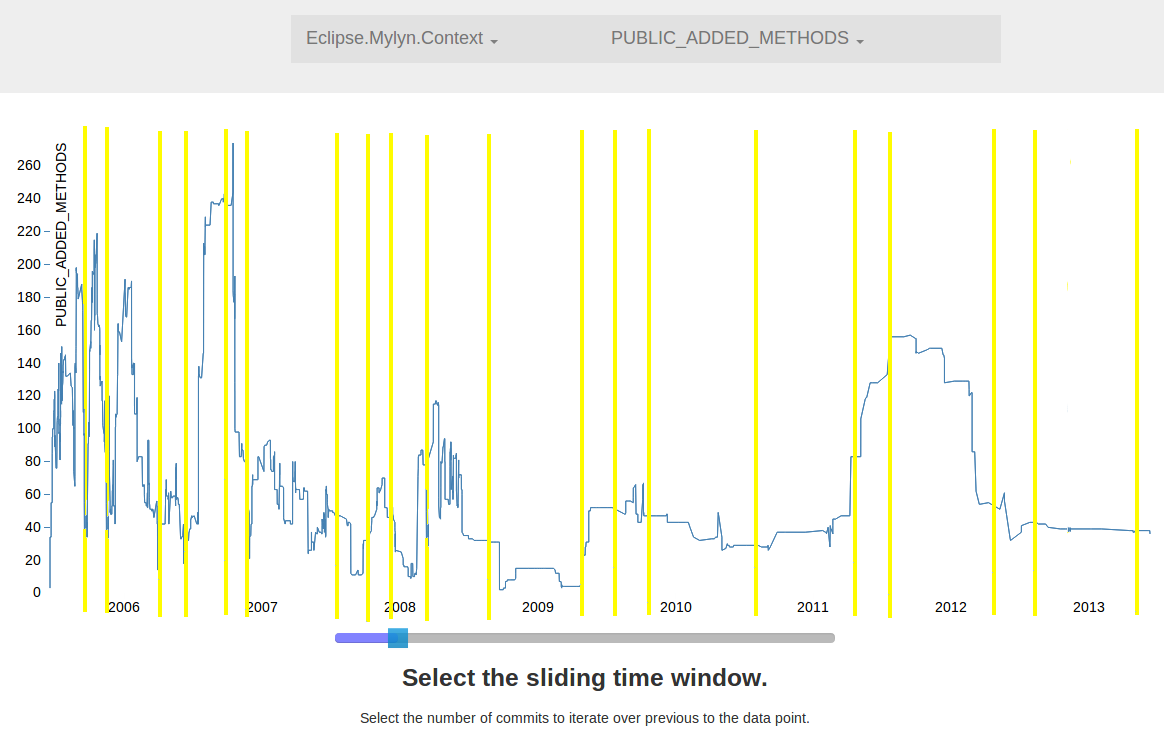
\includegraphics[width=0.5\textwidth]{images/apie.png}
\caption{A screen shot of the APIE visualizer showing project Eclipse.Mylyn.Context with change type PUBLIC\_ADDED\_METHODS being analyzed and showing
major releases as vertical yellow lines.\label{fig:apie}}
\end{figure}

We performed 1888 manual inspections across 10 projects, 472 release dates and 4 change types, and used this data to form the basis of our qualitative data.
Quantitative data was used to compliment the quantitative ratios found from the previous methodology. 

\section{Results}
\label{sec:results}

To answer our research question, we conducted a case study of 10 open source Java projects. These projects are: eclipse.jdt.core, eclipse.jdt.ui, eclipse.jetty.project, 
eclipse.mylyn.commons, eclipse.mylyn.context, hibernate-orm, hibernate-ogm, hibernate-search, eclipse.maven.core, and eclipse.maven.surefire. These project were chosen
because of their high use amongst other Java projects and to study specific ecosystems of projects and their evolution trends.

Due to space requirements of this paper, we focus our results on major releases of the 10 case study projects and select few of the calculated change ratios. 
There were 109 major releases across the 10 studied projects. All of the major findings as per values computed from Equation~\ref{eq:norm} for non test metrics
can be seen in Table~\ref{tab:ratio}.

\begin{table}[h]
\begin{center}
\tabcolsep=0.11cm
\begin{tabular}{| l | c | c | c |}
\hline
Object & Added & Changed & Removed\\
\hline
Public Classes & 1.14 & 0.86 & 1.16 \\
Public Methods (Signature) & 1.07 & 0.92 & 1.34 \\
Public Methods (Bodies) & - & 1.06 & - \\
Private Classes & 0.81 & 1.18 & 1.44 \\
Private Methods (Signatures) & 1.00 & 1.10 & 1.22 \\
Private Methods (Bodies) & - & 1.08 & - \\
Files & 1.12 & 0.96 & 1.14 \\
Documentation & - & 0.99 & - \\
\hline
\end{tabular}
\end{center}
\caption{Implementation oriented change types and their normalized average change ratios at 60 days on each side of releases. \label{tab:ratio}}
\end{table}

To study the most prevalent change trends, we set a ratio threshold of greater than 1.2, or less than 0.83 (20\% greater trend of after the release date
or 20\% greater trend of before the release date) to indicate the greatest trends.

As it can be seen in Table~\ref{tab:ratio}, there are few change type trends around major releases which pass our threshold. We can see that both public
and private methods
being removed from a project is more likely to occur after a major release than after. Table~\ref{tab:ratio} also shows significance in the changes to private
classes. We see that private classes are added more (24\%) before a major release and removed more after (44\%) the release. 
All results in Table~\ref{tab:ratio} could be used as identified trends of major software releases, while we have just highlighted the larger ratios
which meet our threshold criteria in this paper.

Another interesting trend that can been seen in Table~\ref{tab:ratio} is that of changes to public objects. We can see for public classes and methods that
5 out of 7 ratios indicate changes occur to these objects after major release rather than before. We hypothesize that these changes to the public API
after a major release come from newly reported bugs from end users as well as having old features being deprecated while adding new features to the project
after the stable build had been released.

Our complementary qualitative results from manual graph inspections can be seen in Table~\ref{tab:qual}. These results show that adding, changing signatures
and bodies of, and removing public methods tend to all be at a local minimum of change type trends at major releases when activity is not taken into
account. These results confirm previous results of low code churn as an indication of stability.

\begin{table*}[tb!]
\begin{center}
\begin{tabular}{| l | c | c | c | c |}
\hline
Change Type & Upward Trend & Local Maximum & Downward Trend & Local Minimum\\
\hline
Added Public Methods & 21.6\% & 17.2\% & 14.7\% & 33.6\% \\
Changed Public Methods (Signature) & 6.0\% & 19.8\% & 19.0\% & 39.7\% \\
Changed Public Methods (Bodies) & 9.2\% & 16.5\% & 26.6\% & 37.6\% \\
Removed Public Methods & 7.8\% & 16.4\% & 12.9\% & 41.4\% \\
\hline
\end{tabular}
\end{center}
\caption{Qualitative graph analysis results. \label{tab:qual}}
\end{table*}

Lastly we found that software changes related to testing can be an indicator of a major release points within the projects studied. The change
ratios found can be seen in Table~\ref{tab:test}. As it can be seen, the four ratios which meet our threshold and are indicators of stability with regards to test based
changes are: the changing of test classes, the removal of test classes, the adding of methods, and the changing of method signatures, and test classes being changed.
Changes to documentation also meets our threshold and occurs more before a major release.

\begin{table}[h]
\begin{center}
\begin{tabular}{| l | c | c | c |}
\hline
Object & Added & Changed & Removed\\
\hline
Classes & 1.07 & 1.21 & 0.76 \\
Methods (Signatures) & 1.23 & 0.83 & 1.01 \\
Methods (Bodies) & - & 0.90 & - \\
Documentation & - & 0.72 & - \\
\hline
\end{tabular}
\end{center}
\caption{Test oriented change types and their normalized average change ratios at 60 days on each side of releases. \label{tab:test}}
\end{table}

While all change ratios may need to be considered for continued analysis or a taxonomy of change trends, we have offered the strongest
change trends in these results as a suggestion for future focus.

\section{Future Work}
\label{sec:fut}

In future work of change trend analysis, we have planned further statistical tests of the change trends identified in this paper. We would like to
be able to determine if these patterns are unique to major releases versus other types of releases (minor, alpha, beta, release candidate) and to
be able to determine if these pattern are unique to releases alone or can be spotted throughout the history of a project.

If it is deemed that these change trends are present in no other releases, some, all, or in non release history of the project, we will
compare the history of the projects as to where these trends are found against preexisting software stability and quality metrics. We will use this data to
create a new method of discovering when software can be considered stable in reference to the types of software changes being made. 

\section{Conclusions}
\label{sec:con}

Software stability is an often used measure in determining some aspects of code quality. This paper has presented some initial indications as to how
software stability may be found, based on major release stabilities, by analyzing source code change type trends both before and after major software
releases. 

The 4 change trends found in this paper occurring before major releases are: added private classes, changed test method signatures, changed documentation,
and removed test classes.
The 5 change trends found in this paper occurring after major release are: added test methods, changed test classes, removed public methods, removed
private classes, and removed private methods.

The source code change trends found in this paper, in combination with future work and analysis, will allow for the detection of stable code
points throughout a software projects life time. This paper has also shown the beginnings of a visualization for source code change trends which may
be used as a visual cue towards project stability and potential areas of instability where action may need to be taken.

\bibliographystyle{IEEEtran}
%\balance
\bibliography{paper}

% End of the paper
\end{document}
